\documentclass[12pt]{article}
\usepackage[utf8]{inputenc}

\usepackage{mystyle}
\usepackage{parskip}
\usepackage{float}
\usepackage[normalem]{ulem}

% fancy header
\usepackage{fancyhdr}
\pagestyle{fancy}
\rhead{Joseph Sullivan}

\title{A Toric Proof of Pick's Theorem}
\author{Joseph Sullivan}
\date{March 2024}

\DeclareMathOperator{\Ehr}{Ehr}
\DeclareMathOperator{\Area}{Area}
\DeclareMathOperator{\Cone}{Cone}
\DeclareMathOperator{\Relint}{Relint}
\DeclareMathOperator{\Star}{Star}

\begin{document}

\maketitle

\begin{abstract}
    Pick's theorem is a cute result which tells you how to compute the area of a lattice polygon by counting. Though it has much simpler proofs, we use it as an excuse to take a tour through toric geometry. We introduce toric varieties, we sketch some proofs highlighting the correspondence between their combinatorial data and geometry, and finally we deduce Pick's theorem (and more!) by studying the Hilbert polynomial of a divisor associated to our polygon.
\end{abstract}

\tableofcontents

\section{Things to Learn}
\begin{itemize}
    \item Exercises 9.4.2, 9.4.3 to see that Hilbert polynomial is indeed a polynomial
    \item Hartshorne III.2.7
\end{itemize}

\section{Setup}

Pick's theorem is a very cute result in planar geometry. We say a \textbf{polygon} $P$ is a subset of $\R^2$ whose boundary is given a piecewise linear curve. $P$ is said to be \textbf{full-dimensional} if the affine dimension is $2$ (i.e., take any $p\in P$ and take the dimension of the vector space span of the translate $P-p$). $P$ is said to be a \textbf{lattice} polygon if each vertex is in $\Z^2$.

\begin{restatable}[Pick's Theorem]{thm}{pick}\label{thm:pick}
    Let $P\subseteq \R^2$ be a full-dimensional lattice polytope. Let $i=|\mathrm{int}(P) \cap \Z^2|$ count the interior lattice points and $b=|\partial P \cap \Z^2|$ count the lattice points on the boundary. Then,
    \[\Area(P) = i + \frac{1}{2}b - 1.\]
\end{restatable}

We will prove Pick's Theorem by studying the function
\[\ell \longmapsto |\ell P \cap \Z^2|.\]


To prove Ehrhart Reciprocity, we will go through a story regarding toric varieties. At the end of the day, the Ehrhart polynomial will be the Hilbert polynomial of a divisor
\begin{itemize}
    \item Understanding the correspondence between \textit{fans of cones} and normal toric varieties, and then full-dimensional polytopes and normal projective toric varieties.
    \item Understanding torus invariant divisors as rays in a lattice, and combinatorial interpretations of Cartier, ampleness, nef, global sections, etc.
    \item Strong vanishing theorems to compute Hilbert polynomials for nice divisors.
\end{itemize}

\section{Toric Varieties and Fans}

\begin{defn}
    A \textbf{toric variety} is a normal irreducible variety $X$ containing a torus $T=(\C^*)^n$ as a Zariski open subset such that the action of $T$ on itself extends to an algebraic action of $T$ on $X$.
\end{defn}

Some authors do not require normal---we put in this assumption to make the correspondence between the algebraic geometry and combinatorics/convex geometry very sharp.

We will see that toric varieties correspond nicely with combinatorial data, called fans.

\subsection{From Fans to Toric Varieties}

Let $N\cong \Z^n$ be a lattice, and let $N_\R = N\otimes_\Z \R \cong \R^n$ be the $\R$ extension of scalars.

\begin{defn}
    A \textbf{convex polyhedral cone} in $N_\R$ is a subset
    \[\sigma = \Cone(S) = \left\{\sum_{u\in S} \lambda_u u \mid \lambda_u \geq 0\right\} \subseteq N_\R\]
    for a finite subset $S\subseteq N_\R$. In this case, $\sigma$ is called the \textbf{conical hull} of $S$.

    Furthermore, $\sigma$ is called \textbf{rational} if we can take $S\subseteq N$, and \textbf{strictly convex} if $\sigma$ does not contain a line.

    A \textbf{face} of $\sigma$ is an intersection
    \[\sigma \cap H\]
    for some supporting hyperplane $H$. We allow $H=N_\R$ corresponding to the $0$ vector in $N_\R^\vee$, so $\sigma$ is itself a face of $\sigma$. Otherwise, we call $\sigma\cap H$ a \textbf{proper face}.
\end{defn}

We only care about strongly convex rational polyhedral cones, and will mean to include all of the adjectives when we say cone.

For example,

\begin{figure}[H]
\centering
\begin{tikzpicture}[scale=0.5]
    % fill in cone
    \fill[lightgray] (0, 0) -- (3, 1.5) -- (3, 2) -- (0, 2) -- (0, 0);
    
    % draw axes
    \draw[dashed, darkgray] (-1, 0) -- (3, 0);
    \draw[dashed, darkgray] (0, -1) -- (0, 2);
    
    % draw (real) generators
    \draw[thick, ->] (0, 0) -- (0, 1);
    \draw[semithick] (0, 1) -- (0, 2);
    
    \draw[thick, ->] (0, 0) -- (2, 1);
    \draw[semithick] (2, 1) -- (3, 1.5);
    
    % draw labels for generators
    %\draw (0,1) node[anchor=east] {$(0,1)$};
    %\draw (3,-2) node[anchor=north west] {$(3,-2)$};
    
    % draw interior points
    \foreach \x in {-1, ..., 3} {
        \foreach \y in {-1, ..., 2} {
            \fill (\x, \y) circle (0.04in);
        }
    }
\end{tikzpicture}
\caption{Cone in $N_\R$ generated by $e_2$ and $2e_1 + e_2$.}
\end{figure}
is a cone $\Cone(e_2,2e_1+e_2)$ with faces $\Cone(e_2)$, $\Cone(2e_1+e_2)$, and $\Cone(0)$.

Next, a fan is a special type of collections of cones. Just as simplices are to simplicial complexes, cones are to fans.

\begin{defn}
    A \textbf{fan} $\Sigma$ in $N_\R$ is a finite collection of cones $\sigma \subseteq N_\R$ such that
    \begin{enumerate}[(a)]
        \item Every $\sigma\in \Sigma$ is a strongly convex rational polyhedral cone.
        \item For all $\sigma \in \Sigma$, each face of $\sigma$ is also in $\Sigma$.
        \item For all $\sigma_1,\sigma_2 \in \Sigma$, the intersection $\sigma_1 \cap \sigma_2$ is a face of each.
    \end{enumerate}
\end{defn}

For example, the picture

\begin{figure}[H]
    \centering
    \begin{tikzpicture}[scale=0.5]
        % fill in cone
        \fill[color=lightgray] (0,0) -- (3,-2) -- (3,2) -- (0,2) -- (0,0);
        
        % draw axes
        \draw[dashed, color=darkgray] (-1, 0) -- (3, 0);
        \draw[dashed, color=darkgray] (0, -2) -- (0, 2);
        
        % draw (real) generators
        \draw[thick, ->] (0,0) -- (0,1);
        \draw[semithick] (0,0) -- (0,2);
        \draw[thick, ->] (0,0) -- (1,0);
        \draw[semithick] (0,0) -- (3,0);
        \draw[thick, ->] (0,0) -- (3,-2);
        
        % draw interior points
        \foreach \p in {(0,0), (0, 1), (0, 2), (1, 0), (1, 1), (1, 2), (2, -1), (2, 0), (2, 1), (2, 2), (3, -2), (3, -1), (3, 0), (3, 1), (3, 2)} {
            \fill \p circle (0.04in);
        }
    \end{tikzpicture}
    \caption{Fan in $N_\R$}
\end{figure}

corresponds to the fan
\[\Sigma=\{\Cone(e_1,e_2),\Cone(e_1,3e_1-2e_2),\Cone(e_2),\Cone(e_1),\Cone(3e_1-2e_2),\Cone(0)\}.\]

We will then have the correspondence
\[\begin{array}{rcl}
    \text{cones} & \longleftrightarrow & \text{affine toric varieties}\\
    \text{faces} & \longrightarrow & \text{distinguished open sets}\\
    \text{fans} & \longleftrightarrow & \text{toric varieties (glued from affines along distinguished opens)}\\
    \text{origin} & \longleftrightarrow & \text{dense torus}
\end{array}\]

The process for going from a fan to a toric variety will involve two contravariant steps---we will start with our cones, take dual cones which will give us $\C$-algebras, and then take $\Spec$ to get a variety. This initial ``dual'' step might seem redundant/silly, but the effect will be that the total process is covariant. This will also become more clearly desirable when we learn how to recover the fan from a toric variety.

For this dualizing step, we will need to fix $M = N^\vee$ the dual lattice, so $M_\R = N_\R^\vee$.

\subsubsection{Affine Case}

\subsubsection{Constructing the Affine Toric Variety}
Let $\sigma \subseteq N_\R$ be a strongly convex rational polyhedral cone. The \textbf{dual cone} is a cone in $M_\R$
\[\sigma^\vee = \{m\in M_\R \mid \<m,u\> \geq 0 \text{ for all } u\in \sigma\},\]
i.e., the set of all supporting half-spaces. By Farkas' lemma, $\sigma^\vee$ is a convex rational polyhedral cone. We can then intersect $\sigma^\vee$ with the lattice $M\subseteq M_\R$ to get an semigroup
\[\sigma^\vee \cap M_\R,\]
which by Gordan's lemma is finitely generated, so it is an \textbf{affine semigroup} (i.e., commutative, finitely generated, and embedded in a lattice $M$). This will also be \textbf{saturated} in $M$, i.e., if for some $k\in \Z_{>0}$, $km\in S_\sigma$ then $m\in S_\sigma$.

Rather than thinking of elements $m\in S_\sigma \subseteq M\cong \Z^n$ as lattice points which are a semigroup under addition, we will write elements as $\chi^m$ which are a semigroup under multiplication, i.e.,
\[\chi^m \chi^{m'} = \chi^{m+m'}.\]

Now, our facts about $S_\sigma$ will tell us that the semigroup algebra $\C[S_\sigma]$ is a finitely generated (because polyhedral rational) integrally closed (because saturated) domain, so that
\[U_\sigma = \Spec \C[S_\sigma]\]
is a normal affine variety.

As usual, we can characterize (closed) points as maximal ideals, which correspond to ring homomorphisms (due to algebraically closed)
\[\C[S_\sigma] \to \C\]
which (by restricting) correspond to (multiplicative) semigroup homomorphisms
\[S_\sigma \to \C.\]
Essentially, this map is the evaluation map of the point restricted to $S_\sigma$. For a full dimensional cone $\sigma$, this perspective also gives us a distinguished point in $U_\sigma$, which corresponds to the semigroup homomorphism
\begin{align*}
    \gamma_\sigma : S_\sigma &\longrightarrow \C\\
    m &\longmapsto \begin{cases}
        1 & m \in \sigma^\perp\\
        0 & \text{else}
    \end{cases}
\end{align*}
For example, for a full dimensional cone this will be the morphism sending $S_\sigma \to 0$.

\subsubsection{Distinguished Opens}

If $\tau \subseteq \sigma \subseteq N_\R$, then duality flips the inclusion, giving us (following all the steps to construct $U_\tau$ and $U_\sigma$)
\begin{align*}
    \tau^\vee &\supseteq \sigma^\vee\\
    \C[S_\tau] &\supseteq \C[S_\sigma]\\
    U_\tau &\longrightarrow U_\sigma.
\end{align*}

\begin{prop}\label{prop:face_open}
    If $\tau$ is a face of $\sigma$, then $U_\tau \to U_\sigma$ embeds $U_\tau$ as a distinguished open set of $U_\sigma$
\end{prop}

\begin{proof}
    It is true from geometry/combinatorics that
    \[S_\tau = S_\sigma + \Z_{\geq 0} \cdot (-u)\]
    for some $u\in S_\sigma$, e.g.,
    \begin{center}
        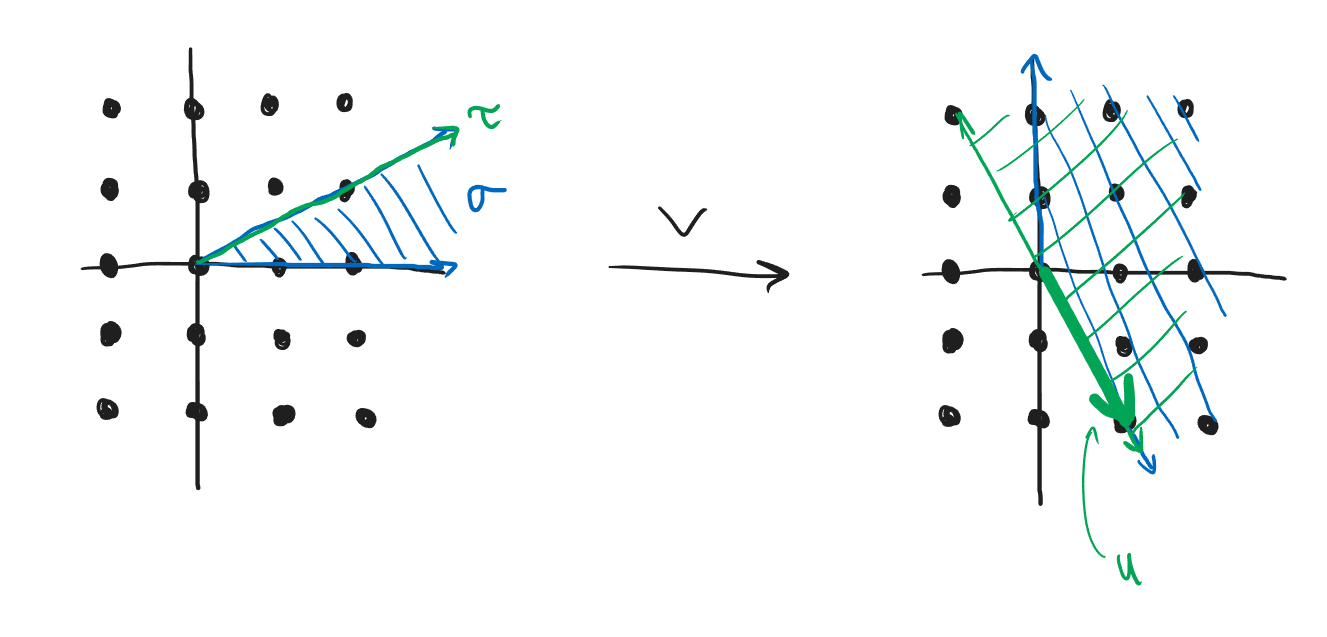
\includegraphics[scale=0.25]{image1.png}
    \end{center}
    Therefore,
    \[\C[S_\sigma] = \C[S_\tau, \chi^{-u}] = \C[S_\tau]_{\chi^{u}},\]
    which implies
    \[\Spec(\C[S_\tau]) = D(\chi^u) \subseteq \Spec(\C[S_\sigma]).\]
\end{proof}

In particular, since $\sigma$ is strictly convex, it has $0$ as a face, and $0^\vee = M_\R$, so $U_{0} = \Spec(\C[M]) \cong (\C^*)^n$ is realized as a distinguished open set of $U_\sigma$. This is exactly the dense open torus.

This also gives us another perspective on $N$. As a set,
\[U_{\{0\}} \cong \Hom(M, \C) = \Hom(M,\C^*) = N\otimes_{\Z} \C^*,\]
since any semigroup homomorphism $M\to \C$ lands in $\C^*$ (since $\chi^{-m}$ is sent to $(\chi^m)^{-1}$). In light of this, we denote the torus by $T_N$.

In this way, given a fan $\Sigma$ we get a prevariety $X_\Sigma$ (a-priori we don't know if its separated yet) as the pushout of the inclusions of these affine open sets. That is, we disjoint union every $U_\sigma$, and we glue along inclusions of common faces $U_{\sigma\cap \tau}$ to $U_\sigma$, $U_\tau$.

Then, to show $X_\Sigma$ is separated, we need the following lemma.
\begin{lem}
    If $\sigma$ and $\tau$ are cones that intersect at a common face, then the diagonal map
    \[U_{\sigma \cap \tau} \to U_\sigma \times U_\tau\]
    is a closed embedding.
\end{lem}

\begin{proof}
    This is equivalent to showing
    \begin{align*}
        \Delta^*: \C[S_\sigma] \otimes_\C \C[S_\tau] &\longrightarrow \C[S_{\sigma\cap \tau}]\\
        \chi^m \otimes \chi^{m'} &\longmapsto \chi^{m+m'} 
    \end{align*}
    is surjective, i.e., we want to see that every function on $U_{\sigma\cap \tau}$ is the product of restrictions of functions on $U_\sigma$, $U_\tau$. This corresponds to seeing if every $\chi{m''}\in S_{\sigma\cap \tau}$ can be obtained as the product of $\chi^m\in S_\sigma$ and $\chi^{m'}\in S_\tau$. Finally, this is equivalent to the statement
    \[S_{\sigma \cap \tau} = S_\sigma + S_\tau,\]
    which is fact called the \textit{Separation Lemma}, which we will not prove.
\end{proof}

Now, this implies $X_\Sigma$ is separated because the diagonal $\Delta: X_\Sigma \to X_\Sigma \times X_\Sigma$ is a closed embedding, since we have an open cover
\[\{U_\sigma \times U_\tau\}_{\sigma,\tau \in \Sigma}\]
such that the diagonal restricted to $\Delta^{-1}(U_\sigma\times U_\tau)$ is a closed embedding by the lemma.

So, we see that $X_\Sigma$ is indeed a (normal) variety, and it has a dense open torus $T_N$. To see that $X_\Sigma$ is a toric variety, we are only missing the torus action.

\subsubsection{Torus Action}

As we mentioned before, a point on the torus $T_N$ corresponds to a map $t:M\to \C^*$. Now, for a point $x\in U_\sigma$ corresponding to $x: S_\sigma\to \C$, define $t\cdot x$ as the point corresponding to the map $S_\sigma \to \C$ by
\[u \longmapsto t(u)x(u) \in \C.\]
The dual map on algebras is by pulling back, so plugging in $t\cdot x$ for $\chi^m$ we can deduce
\begin{align*}
    \C[S_\sigma] &\longrightarrow \C[M]\otimes_\C \C[S_\sigma]\\
    \chi^m &\longmapsto \chi^m \otimes \chi^m.
\end{align*}

\begin{prop}\label{prop:fixed_pt}
    If $\sigma$ is a full-dimensional cone in $\Sigma$, then the distinguished point $\gamma_\sigma$ is the unique fixed point of the torus action. For $\sigma$ not full-dimensional, there are no fixed points.
\end{prop}

\begin{proof}
    A point $x\in U_\sigma$ is a fixed point exactly when as a homomorphism $S_\sigma \to \C$, it maps all $\chi^m$ for $m\neq 0$ to $0$ (every homomorphism must map $0\in M$ to $1$ to be a semigroup homomorphism). Otherwise, we could find $t\in T_N$ which doesn't fix $x$ by mapping for example $m\mapsto 2$ (do this by choosing a minimal generator of $\R m \cap M$ and completing this to a $\Z$-basis of $M$). Then, $t\cdot x$ maps $\chi^m \mapsto 2$, so we get a distinct point.

    So, for $\sigma$ a full-dimensional cone, we can indeed map every $\chi^m$ for $m\neq 0$ and $m\in S_\sigma$ to $0$, since $-m\not\in S_\sigma$ (i.e., $\sigma^\perp = \{0\}$, or $\sigma^\vee$ is strictly convex). This is exactly the distinguished point, and by our discussion it is our unique fixed point.
    
    On the other hand, if $\sigma$ is not full-dimensional, there exist minimal $\pm m\in \sigma^\perp\cap M$, corresponding to functions $\chi^{\pm m}$ on $U_\sigma$. Then, every very point $x\in U_\sigma$ as a homomorphism $S_\sigma \to \C$ must map $\pm m$ to a nonzero point (in order to be a semigroup homomorphism). By our previous discussion, this implies $x$ is not fixed, so $U_\sigma$ has no fixed point.
\end{proof}

This is one good reason to study the distinguished points, at least for full dimensional cones. We can more naturally arrive at these distinguished points by studying limits of 1-parameter subgroups. A point $u=(b_1,\dots,b_n)\in N$ is exactly a 1-parameter subgroup
\[\lambda^u: t \mapsto (t^{b_1},\dots,t^{b_n})\]
of $T_N$. In general, $\lambda^u(t)$ won't converge in $T_N$ when we send $t\to 0$, except for $u=0$. However, in a toric variety (many of which are compactifications of $T_N$), many of these limits do converge. We characterize when and where.

{\color{red} example of $\P^2$}

\begin{prop}
    Let $\sigma\subseteq N_\R$ be a strongly convex rational polyhedral cone and let $u\in N$. Then
    \[u\in \sigma \quad \iff \quad \lim_{t\to 0} \lambda^u(t) \text{ exists in $U_\sigma$}.\]
    Moreover, if $u\in \Relint(\sigma)$, then $\lim_{t\to 0}\lambda^u(t) = \gamma_\sigma$.
\end{prop}

\begin{proof}
    Given $u\in N$, we have
    \begin{align*}
        \lim_{t\to 0} \lambda^u(t) \text{ exists in $U_\sigma$} &\iff \lim_{t\to 0} \chi^m(\lambda^u(t)) \text{ exists in $\C$ for all } m\in S_\sigma\\
        &\iff \lim_{t\to 0} t^{\<m,u\>}  \text{ exists in $\C$ for all } m\in S_\sigma\\
        &\iff \<m,u\>\geq 0  \text{ for all } m\in \sigma^\vee \cap M\\
        &\iff u\in (\sigma^\vee)^\vee=\sigma,
    \end{align*}
    (first assertion is because the $\chi^m$ are coordinates for a generating set of $S_\sigma$, so limit exists iff coordinate limits exist). Then, this limit is given by (for $m\in S_\sigma$)
    \[m\mapsto \lim_{t\to 0} t^{\<m,u\>},\]
    so for $u\in \Relint(\sigma)$, we have $\<m,u\>>0$ for $m\not\in \sigma^\perp$, so
    \[m\mapsto \begin{cases}
        1 & m\in \sigma^\perp\\
        0 & \text{else}
    \end{cases},\]
    so indeed this is the distinguished point $\gamma_\sigma$.
\end{proof}

\subsection{Orbit-Cone Correspondence}

We saw in Proposition \ref{prop:fixed_pt} that for a full-dimensional cone $\sigma$, the distinguished point $\gamma_\sigma$ is a fixed point, so in particular an orbit. We also understand another orbit, which is the torus itself $T_N$. We now want to understand all of the orbits.

We will define
\[O(\sigma) = T_N \cdot \gamma_\sigma.\]
We will see that this orbit is a torus of lower dimension. Define
\begin{align*}
    N_\sigma &= \Z\cdot(\sigma\cap N),\\
    N(\sigma) &= N/N_\sigma.
\end{align*}
We will see that that $T_{N_\sigma}$ is the kernel of the action of $T_N$ on $O(\sigma)$, so that $T_{N(\sigma)}$ acts faithfully. Even more, it acts freely.
\begin{lem}
    Let $\sigma$ be a SCRP cone in $N_\R$. Then,
    \begin{align*}
        O(\sigma) &= \{\gamma: S_\sigma \to \C \mid \gamma(m)\neq 0 \iff m\in \sigma^\perp \cap M\}\\
        &\cong \Hom_\Z(\sigma^\perp \cap M, \C^*)\\
        &\cong T_{N(\sigma)}.
    \end{align*}
\end{lem}

\begin{thm}[Orbit-Cone Correspondence]\label{thm:orbit_cone}
    Let $X_\Sigma$ be the toric variety of the fan $\Sigma$ in $N_\R$. Then:
    \begin{enumerate}[(a)]
        \item There is a bijective correspondence
        \begin{align*}
            \{\text{cones in }\Sigma\} &\longleftrightarrow \{\text{$T_N$-orbits in $X_\Sigma$}\}\\
            \sigma &\longleftrightarrow O(\sigma)
        \end{align*}
        \item Let $n=\dim N_\R$. Then for each $\sigma\in \Sigma$, $\dim O(\sigma) = n-\dim \sigma$.
        \item The affine open subset $U_\sigma$ is the union of orbits
        \[U_\sigma = \bigcup_{\tau\preceq \sigma} O(\tau).\]
        \item $\tau\leq \sigma$ iff $O(\sigma) \subseteq \overline{O(\tau)}$, and
        \[\overline{O(\tau)} = \bigcup_{\tau\preceq \sigma} O(\sigma),\]
        where $\overline{O(\tau)}$ denotes the closure in both the classical and Zariski topologies.
    \end{enumerate}
\end{thm}

In particular, $\overline{O(\tau)}$ is a subvariety, and even more a toric variety. Define
\[\Star(\tau) = \{\overline{\sigma}\subseteq N(\tau)_\R \mid \tau\preceq \sigma \in \Sigma\}\]
where $\overline{\sigma}$ is the image in the quotient. Then, $\Star(\tau)$ is a fan in $N(\tau)_\R$, and
\[\overline{O(\tau)} \cong X_{\Star(\tau)}.\]
\subsection{From Toric Varieties to Fans}

Now, given a (normal) toric variety $X$, we want to recover the fan $\Sigma$. Some things that suggest this is possible (at least from toric varieties are constructed from fans, i.e., $X=X_\Sigma$) is that orbits of the torus action lie inside these $U_\sigma$ by construction. Full-dimensional cones also have these unique fixed points corresponding to them.

We can at least recover the lattices $N$ and $M$ by considering
\[N= \Hom(\C^*, T) = \{t \mapsto (t^{a_1},\dots,t^{a_n}) \mid a_1,\dots,a_n\in \Z^n\} \cong \Z^n\]
\[M= \Hom(T, \C^*) = \{(t_1,\dots,t_n) \mapsto t_1^{b_1}\cdots t_n^{b_n} \mid b_1,\dots,b_n\in \Z^n\} \cong \Z^n.\]
We have a pairing $N\times M \to \Z$ by considering the composition $\C^* \to T \to \C^*$ (since $\Hom(\C^*,\C^*)=\Z$), and this pairing is perfect, expressing $N,M$ as duals of each other.

Now, we want to find the fan inside $N$. We blackbox a theorem from algebraic groups.
\begin{thm}[Sumihiro]
    Let the torus $T$ act on a normal separated variety $X$. Then every point $p\in X$ has a $T$-invariant affine open neighborhood.
\end{thm}

This theorem crucially uses the normal hypothesis, this is one place where the assumption comes into play (and it must come into play because every $X_\Sigma$ is normal, and not all toric varieties are normal).

So, we have a cover of $X$ by normal affine toric varieties. So, we will show that every normal affine toric variety $U$ with torus $T_N$ comes from a (strictly convex rational polyhedral) cone $\sigma_U \subseteq N_\R$, and we will set
\[\Sigma_X = \{\sigma_U \mid U \text{ is an affine toric variety in } X\}.\]
So, to see that $\Sigma_X$ is a fan, we already have (a), and (b) follows from Proposition \ref{prop:face_open}. We just have to check (c), so we will need to see that
\[\sigma_{U\cap V} = \sigma_U \cap \sigma_V.\]

\subsubsection{Affine Case}
Now, to find the cone corresponding to a toric variety, we first need a result from algebraic groups (this is true for any diagonalizeable algebraic group, but we only focus on the torus). We will see that the coordinate ring $\C[U]$ of an affine toric variety is a subalgebra of $\C[M]$, but to get that it is generated by an affine monoid we need the following result.
\begin{lem}\label{lem:rational_torus_reps}
    Let $T=(\C^*)^n$ act linearly on a finite dimensional vector space $W$, i.e., we have a homomorphism $\phi: T\to \GL(W)$ of algebraic groups. Then, we can simultaneously diagonalize all $\phi(t)$, i.e., choose one basis for $W$ that diagonalizes all $\phi(t)$. Even more, the eigenspaces will be of the form
    \[W_m = \{w\in W \mid \phi(t)w = \chi^m(t) w \text{ for all } t\in T\}\]
    for some finite collection of $m\in M$.
\end{lem}

This result will use Dedekind's theorem on characters.
\begin{thm}[Dedekind]
    Let $\chi_1,\dots,\chi_n: G\to \C^*$ be distinct characters (group homomorphisms). Then, they are linearly independent (in the vector space of set functions $G\to \C$ with pointwise scaling).
\end{thm}

\begin{proof}[Proof of lemma.]
    If we did have a simultaneously diagonalization of $W\cong \C^k$, then we would be able to write $\phi$ as
    \[t \mapsto P\begin{bmatrix}
        \phi_1(t) & & \\
         & \ddots & \\
         & & \phi_k(t)
    \end{bmatrix}P^{-1},\]
    and since $\phi$ is an algebraic group homomorphism, this will force every $\phi_i$ to be an algebraic group homomorphism $T \to \C^*$, i.e., a character $\chi^m\in M$, and the eigenvalues of $\phi(t)$ will be $\chi^{m_1}(t),\dots,\chi^{m_k}(t)$. So, for varying $t$, each $\phi(t)$ will have different eigenvalues (they vary with $t$), but it turns out that for a fixed $\chi^m$, the eigenspace of eigenvalue $\chi^m(t)$ will be a constant subspace of $W$ (does not depend on $t$).

    Motivated by this, we will define
    \[W_m = \{w\in W \mid \phi(t)w = \chi^m(t)w \text{ for all } t\in T\}.\]
    We will expect (hope) that all but finitely many $W_m$ are nonzero, and that the remaining $W_m$ will sum up to $W$.

    To see this, note that $\pi_{ij}\circ \phi: T \to \C$ is a regular map, and regular maps from the torus are sums of characters. So, $\phi$ is a matrix with entries which are sums of characters as functions of $t$. Splitting $\phi(t)$ into sums and factoring out common characters, we get a finitely supported 
    \[\phi(t) = \sum_{m \in M} \chi^m A_m,\]
    where $A_m \in \C^{n\times n}$ is some constant matrix. Since $\phi$ is a group homomorphism, we have
    \[\phi(tt') = \phi(t)\phi(t'),\]
    and expanding both sides we get
    \begin{align*}
        \sum_{m\in M} \chi^m(t) \chi^m(t') A_m &= \left(\sum_{m\in M} \chi^m(t) A_m\right)\left(\sum_{m'\in M} \chi^{m'}(t') A_{m'}\right)\\
        &= \sum_{m,m'\in M} \chi^m(t) \chi^{m'}(t') A_m A_{m'}.
    \end{align*}
    Then, each coordinate (i.e., after projecting with some $\pi_{ij}$) is a sum of distinct characters $\chi^m \oplus \chi^{m'}$ of $T\times T$. By Dedekind's theorem, distinct characters are linearly independent, so equating coefficients (the $A_m$ and $A_m A_{m'}$), we get
    \[A_m A_{m'} = \delta_{m,m'} A_m,\]
    so they are disjoint and idempotent. This tells us that $\im A_m \subseteq W_m$ (i.e., try applying $\phi(t)$ to $A_m(w)$). Next, evaluating $\phi(1)$ gives us
    \[1 = \sum_{m\in M} A_m,\]
    so $\bigoplus_{m\in M} \im A_m = W$, so $\im A_m = W_m$. So, we indeed get $W$ as this direct sum of eigenspaces that do not depend on $t$.
\end{proof}

\begin{prop}
    Let $U$ be a normal affine toric variety with torus $T_N$. Then, $U=\Spec(\C[S_\sigma])$ for a (strictly convex rational polyhedral) cone $\sigma\subseteq N_\R$.
\end{prop}

\begin{proof}
    The inclusion $T_N \hookrightarrow U$ of a dense open subset induces an injection
    \[\C[U] \hookrightarrow \C[M]\]
    (writing $\C[U]$ for the coordinate ring of $U$, $\C[M]$ the coordinate ring of $T_N$). Our first step is to show $\C[U]$ is actually generated by monomials, so that $\C[U] = \C[S]$ for some affine semigroup $S$. Then, we will use normality to argue that $S=S_\sigma$ for some $\sigma \subseteq N_\R$.

    To find the affine semigroup, we need to use the $T_N$ action. On the level of $T_N$, every $t$ gives a left translation $L_{t^{-1}}: T_N \to T_N$, which corresponds to
    \begin{align*}
        (L_{t^{-1}})^*: \C[M] &\longrightarrow \C[M]\\
        (p\mapsto f(p)) &\longmapsto (p\mapsto f(t^{-1} p))
    \end{align*}
    giving an action of $T_N$ on $\C[M]$. Since $U$ is a toric variety, the action of $T_N$ on $U$ restricts to the usual multiplication in $T_N$. Dually, the action of $T_N$ on $\C[M]$ restricts to the action on $\C[U]$, so we get that $\C[U]$ is closed under the $T_N$ action. Define the subspace
    \[A = \bigoplus_{\chi^m \in \C[U]} \C\cdot \chi^m.\]
    Clearly $A\subseteq \C[U]$. We show equality. Take $f\in \C[U]$ nonzero, which we can write as a linear combination of some monomials $\chi^m$ for $m$ in a finite set $\cB$, i.e.,
    \[f = \sum_{m\in \cB} c_m \chi^m,\]
    and take $\cB$ minimal so that every $c_m\neq 0$. We want to show every monomial $\chi^m \in \C[U]$. Define
    \[B = \bigoplus_{m\in \cB} \C\cdot \chi^m\]
    the vector space span. We can compute
    \[t\cdot \chi^m = \chi^m(t^{-1}) \chi^m\]
    (where $\chi^m(t^{-1})\in \C$), so in particular $B$ is $T_N$ stable. Therefore, $\C[U]\cap B$ is $T_N$-stable and a finite dimensional vector space. By our lemma, this means
    \[\C[U]\cap B = \bigoplus (\C[U] \cap B)_m,\]
    where the eigenspaces $W_m$ consist of exactly the functions $g$ where $t\cdot g = \chi^m(t) g$, which forces $g=\chi^m$. This tells us that $\C[U]\cap B = B$, so $B\subseteq \C[U]$.

    Therefore, $\C[U]$ is generated by monomials, and since $\C[U]$ is finitely generated (since $U$ is a variety), we can do it with finitely many (i.e., take the finitely many generators, and generate each with finitely many monomials). This gives us an affine semigroup $S$ where $\C[U]=\C[S]$.

    We next want to see that $S=S_\sigma$, so we want to see that $S=\tau \cap M$ for some (full-dimensional convex rational polyhedral cone) $\tau$, and then we can take $\sigma = \tau^\vee$ (getting a strictly convex rational polyhedral cone).

    This is where the normal hypothesis gets used. We will show that $S$ is \textbf{saturated}, that if $km\in S$, then $m\in S$. Since $T_N$ is dense in $U$, $\chi^m$ is a rational function on $U$ (a priori maybe not regular), so $\chi^m \in \C(U)$. However, $\chi^m$ is then a root of
    \[t^k - \chi^{km} \in \C[V][t],\]
    so because $\C[V]$ is normal, we need $m \in S$. This then implies that
    \[S = \tau \cap M\]
    where $\tau = \Cone(S)$ (which is a rational polyhedral convex cone by earlier discussion), and $\tau$ is full-dimensional because otherwise $V$ would have smaller dimension (so it couldn't have $T_N$ inside).
\end{proof}

\subsubsection{Distinguished Opens}



At this point, 

do exercise 3.2.2., 3.2.10., 3.2.11.
maybe redo the previous section in light of these? maybe there's something more direct if we can already recover the cone.

\section{Divisors}

We now describe $T_N$-invariant divisors on a toric variety $X_\Sigma$. From our study of orbits, the $T_N$-invariant prime divisors are exactly
\[D_\rho = \overline{O(\rho)}\]
for $\rho \in \Sigma(1)$, where $\Sigma(1)$ denotes the 1-dimensional cones in $\Sigma$. More generally, every $T_N$-invariant Weil divisor is of the form
\[\sum_{\rho\in \Sigma(1)} a_\rho D_\rho\]
for some coefficients $a_\rho \in \Z$.

\subsection{Divisor of a Character}
Our hope is going to be that every linear equivalence class of a Weil divisor is represented by a $T_N$-invariant Weil divisor (which we now understand). However, many $T_N$-invariant Weil divisors will be linearly equivalent, and the hope is going to be that such linear equivalence is expressed exactly by the rational functions on $X_\Sigma$ that we understand the best, namely the characters $\chi^m$. These are indeed rational functions, since they are regular at least on the open set $T_N$.

So, we want to compute $\div(\chi^m)$. Expecting that this will be a formal sum of $D_\rho$, we study its order of vanishing along $D_\rho$. Denote $v_\rho = v_{D_\rho}: \C(X_\Sigma)^* \to \Z$.

\begin{prop}
    Let $X_\Sigma$ be the toric variety of a fan $\Sigma$. If the ray $\rho\in \Sigma(1)$ has minimal generator $u_\rho$ and $\chi^m$ is the character corresponding to $m\in M$, then
    \[v_\rho(\chi^m) = \<m, u_\rho\>.\]
\end{prop}

\begin{proof}
    Since $u_\rho \in N$ is primitive, we can extend $u_\rho$ to a basis $e_1 = u_p$, $e_2,\dots,e_n$ of $N$, then we can assume $N=\Z^n$ and $\rho = $.
\end{proof}


\section{Vanishing Theorems}

\begin{thm}[Demazure Vanishing] \label{thm:demazure}
    Let $D$ be a $\Q$-Cartier divisor on $X_\Sigma$. If $|\Sigma|$ is convex and $D$ if nef, then
    \[H^p(X_\Sigma, \cO_{X_\Sigma}(D)) = 0 \quad \text{for all $p>0$}.\]
\end{thm}

\begin{thm}[Batyrev-Borisov Vanishing] \label{thm:batyrev}
    Let $D = \sum_\rho a_\rho D_\rho$ be a $\Q$-Cartier divisor on a complete toric variety $X_\Sigma$. If $D$ is nef, then
    \begin{enumerate}[(a)]
        \item $H^p(X_\Sigma, \cO_{X_\Sigma}(-D))=0$ for all $p\neq \dim P_D$.
        \item When $p=\dim P_D$, $H^p(X_\Sigma, \cO_{X_\Sigma}(-D))\cong \bigoplus_{m\in\Relint(P_D)\cap M} \C\cdot \chi^{-m}$
    \end{enumerate}
\end{thm}

\section{Divisors on Toric Varieties}

{\color{red} define polyhedron (not polytope because potentially unbounded) $P_D$.}

\begin{prop}\label{prop:global_sections}
    If $D$ is a $T_N$-invariant Weil divisor on $X_\Sigma$, then
    \[\Gamma(X_\Sigma, \cO_{X_\Sigma}(D)) = \bigoplus_{m\in P_D \cap M} \C\otimes \chi^m.\]
\end{prop}

\begin{proof}
    {\color{red} See proposition 4.3.3}
\end{proof}

\section{Ehrhart Reciprocity}

\begin{defn}
    Let $\cF$ be a coherent sheaf on a complete variety $X$. Its \textbf{Euler characteristic} $\chi(\cF)$ is defined to be the alternating sum
    \[\chi(\cF) = \sum_{p\geq 0} (-1)^p \dim H^p(X,\cF).\]
    This is well-defined because coherent+complete implies $\dim H^p(X,\cF)<\infty$ for all $p$, and $H^p(X,\cF)=0$ for $p>\dim X$ by \cite[Thm. III.2.7]{hartshorne}.
\end{defn}

\begin{prop}
    Let $\cF$ be a coherent sheaf on a complete variety $X$ and let $D$ be an ample divisor. Then, the the function
    \[\ell \longmapsto \chi(\cF(\ell D))\]
    is a polynomial, called the \textbf{Hilbert polynomial} of $\cF$.
\end{prop}

In particular, for a projective variety $X$, the Hilbert polynomial of $\cO_X(1)$ is \textit{the} Hilbert polynomial of $X$.

The following theorem finally brings us back to our initial goal of studying the function $\ell \mapsto |\ell P \cap \Z^2|$ for a lattice polygon $P$.

\begin{thm}[Ehrhart Reciprocity]\label{thm:ehrhart}
    Let $P\subseteq \R^n$ be a full-dimensional lattice polytope. There is a polynomial $\Ehr_P(x)\in \Q[x]$ called the \textbf{Ehrhart polynomial} satisfying for $\ell \in \Z_{\geq 0}$,
    \[\Ehr_P(\ell) = |\ell P \cap \Z^n|\]
    and for $\ell \in \Z_{>0}$, then
    \[\Ehr_P(-\ell) = (-1)^n |\mathrm{int}(\ell P) \cap \Z^n|.\]
\end{thm}

In words, counting the lattice points of the $\ell$th scale of $P$ is a polynomial in $\ell$, and more.

\begin{proof}
    Let $X_P$ be the toric variety of $P$ and $D_P$ the associated ample divisor. We will show that the Hilbert polynomial
    \[\ell \mapsto \chi(\cO_{X_P}(\ell D_p))\]
    has the desired properties for $\Ehr_P$.
    
    First, we concern ourselves with nonnegative $\ell\geq 0$.{\color{red} argue $D_P$ meets hypotheses of Demazure vanishing}. Therefore, by Demazure vanishing only the 0th cohomology does not vanish, so
    \[\chi(\cO_{X_p}(\ell D_P)) = \dim H^0(X_P, \cO_{X_P}(\ell D_P)) = \dim \Gamma(X_P, \cO_{X_P}(\ell D_P)),\]
    and by proposition \ref{prop:global_sections} as well as the computations $P_{D_P}=P$ and $\ell D_P = D_{\ell P}$, we get
    \[\dim \Gamma(X_P, \cO_{X_P}(\ell D_P)) = |\ell P \cap M|.\]

    Now, we handle the negative case. Assume $\ell > 0$. {\color{red} argue Batyrev-Borisov vanishing applies}. Therefore, we have
    \[\chi(\cO_{X_P}(-\ell D_P)) = (-1)^n H^p(X_P, \cO_{X_P}(-\ell D_P)) = (-1)^n |\mathrm{int}(\ell P) \cap M|.\]
\end{proof}

{\color{red}\begin{itemize}
    \item figure out what happens for $D=0$ (is this nef/$\Q$-Cartier? does it meet the hypotheses, or are things just trivial?)
    \item why is $D_P$ $\Q$-Cartier, and $|\Sigma_P|$ convex, and $D_P$ nef?  see prop 6.1.10
    \item Why is $P_{D_P} = P$, $P_{kD} = kP_D$?
\end{itemize}}

Now, we can derive Pick's theorem as a corollary. We recall
\pick*

\begin{proof}
    Assume by triangulation the $P$ is convex, so that it is a lattice polytope in $\R^2$. Therefore, Ehrhart reciprocity applies and we get the polynomial $\Ehr_P(x)\in \Q[x]$. We now figure out the degree/coefficients.
    
    From measure theory (by bounding with boxes inside and out)
    \[\Area(P) = \lim_{\ell\to \infty} \frac{|\ell P \cap \Z^2|}{\ell^2} = \lim_{\ell\to\infty} \frac{\Ehr_P(\ell)}{\ell^2}\]
    which tells us $\Ehr_P$ is degree $2$ and has leading coefficient $\Area(P)$.

    Furthermore, $\Ehr_P(0) = |0P\cap \Z^2| = |\{0\}|=1$, so the constant term is $1$. Therefore,
    \[\Ehr_P(x) = \Area(P)x^2 + bx + 1.\]

    Now, plugging in $1$ and $-1$ we get
    \begin{align*}
        \Ehr_P(1) = |P\cap \Z^2| &= \Area(P) + b + 1\\
        \Ehr_P(-1) = |\mathrm{int}(P) \cap \Z^2| &= \Area(P) - b + 1,
    \end{align*}
    so subtracting we get
    \[|\partial P \cap \Z^2| = 2b,\]
    so
    \[\Ehr_P(x) = \Area(P)x^2 + \frac{1}{2}|\partial P \cap \Z^2| + 1.\]
    Plugging in $-1$ and solving for $\Area(P)$, we get Pick's theorem.
\end{proof}


\nocite{*} % Include all references in refs.bib regardless of whether they are referenced or not
\bibliographystyle{plain} % We choose the "plain" reference style
\bibliography{2023spring/toric_pick/toric_pick_refs} % Entries are in the refs.bib file

\end{document}